\documentclass[12pt]{exam}
\usepackage[utf8]{inputenc}

\usepackage{tikz}
\usepackage{pgfplots}

\usetikzlibrary{math}
%\usetikzlibrary{datavisualization.formats.functions}
%\usetikzlibrary{datavisualization}
\usetikzlibrary{intersections}
\pgfplotsset{compat=1.16}


\usepackage{xcolor}
\usepackage{colortbl}
\usepackage{amsmath}
\usepackage{amssymb}
\usepackage{gnuplottex}
\usepackage{graphicx}
\usepackage{siunitx}
\usepackage{multicol}
\usepackage{tasks}
\usepackage{physics}
\usepackage{cancel}
\usepackage{todonotes}
\usepackage{romannum}

\renewcommand{\solutiontitle}{\noindent\textbf{Lösung:}\par\noindent}

\renewcommand{\questionshook}{%
\setlength{\leftmargin}{0pt}%
\setlength{\labelwidth}{-\labelsep}%
}

\newcommand{\uuline}[1]{\underline{\underline{~#1~}}}

\setlength{\jot}{8pt}

\settasks{
    label-width = 11.0971pt
  }


%%%%%%%%% Ausgabe der Lösungen %%%%%%%%%

%\noprintanswers
\printanswers

%%%%%%%%% Rahmen um Lösung %%%%%%%%%
\unframedsolutions
%\framedsolutions

\begin{document}

%%%%%%%%% Grundlegende Einstellungen %%%%%%%%%
%%%%%%%%%   Header - Footer          %%%%%%%%%

\pagestyle{headandfoot}

\firstpageheader{Übungsaufgaben\\ Bodendynamik}{TU Bergakademie Freiberg \\Institut für Geotechnik}{Seite \thepage\ von \numpages\\}
\firstpageheadrule

\firstpagefooter{}{}{}
\runningfooter{}{}{}

\runningheader{Übungsaufgaben\\ Bodendynamik}{TU Bergakademie Freiberg \\Institut für Geotechnik}{Seite \thepage\ von \numpages\\}
\runningheadrule
\runningfootrule

\setlength{\jot}{8pt}


%%% Todonotes margin - remove when done
\setlength {\marginparwidth }{2cm}

\huge\centering Übungsaufgaben Bodendynamik - SS \the\year
\normalsize

\begin{questions}
\section{Grundlagen}
\subsection{Simulation}


    %%%%%%%%% Übungsaufgabe 1 %%%%%%%%%
    
    \question{erzwungene, ungedämpfte Schwingung}
    \vspace{1em}
 
    \begin{minipage}[t]{.49\linewidth}
    geg.:
    \begin{tasks}(2)
       \task[] $m = \SI{3}{\kilo\gram}$
       \task[] $k = \SI{10}{\newton\per\meter}$
        \task[] $F(t) = \hat{F} \sin{\omega t}$
       \task[] $\hat{F} = \SI{5}{\newton}$
       \task[] $\omega = \SI{10}{\radian\per\second}$
       \task[] $t=\SI{0}{\second}$
       \task[] $u_0 = \SI{0.1}{m}$
       \task[] $\dot{u}_0 = \SI{0}{\meter\per\second}$
    \end{tasks}
    \end{minipage}
    \begin{minipage}[t]{.49\linewidth}
    ges.:
    \begin{tasks}
        \task $u(t)$
    \end{tasks}
    \end{minipage}
 
    \begin{solution}
    \begin{alignat*}{2}
        &(c = \SI{0}{\newton\second\per\meter}, F_C = \SI{0}{\newton}, F_S = \hat{F} = \SI{5}{\newton})\\
        &\omega_0 = \sqrt{k/m} &&= \SI{1.826}{\radian\per\second} \\
        &\zeta = \frac{c}{2\sqrt{k/m}} &&= 0 \\
        &\eta = \omega/\omega_0 &&= 5.477\\
        &V = (1-\eta^2)^{-1} &&=  0.0345 \\
        &u_C = -2V^2\zeta\eta\hat{F}/k &&= \SI{0}{\meter} \\
        &u_S = V^2(1-\eta^2)\hat{F}/k &&= \SI{-0.0172}{\meter}
    \end{alignat*}
    
    \begin{align*}
        u_0 &= C_1 + u_C \\
        \dot{u}_0 &= \omega_0 C_2+\omega u_S\\
        &\rightsquigarrow \\
        C_1 &=  u_0 - U_C = \SI{0.1}{\meter}\\
        C_2 &= \frac{\dot{u}_0 - \omega u_S}{\omega_0} = \SI{0.0944}{\meter} \\
        \vspace{1cm}
        \end{align*}
        \begin{equation*}
            \begin{split}
        u(t) = \SI{0.1}{\meter} \cos{(\SI{1.826}{\radian\per\second} t)} +\SI{0.0944}{\meter} \sin{((\SI{1.826}{\radian\per\second} t))} \\ - \SI{0.0172}{\meter}\sin{(\SI{10}{\radian\per\second} t)}
        \end{split}
        \end{equation*}
        \fbox{\textbf{Anmerkung:} Das Einschwingen dauert im  ungedämpften Fall unendlich lang.}
    \end{solution}
 
    %%%%%%%%% Übungsaufgabe 2 %%%%%%%%%
 
    \question{erzwungene, gedämpfte Schwingung}

     \begin{minipage}[t]{.49\linewidth}
        geg.:
        \begin{tasks}(2)
           \task[] $m = \SI{3}{\kilo\gram}$
           \task[] $c = \SI{1}{\newton\second\per\meter}$
           \task[] $k = \SI{10}{\newton\per\meter}$
            \task[] $F(t) = \hat{F} \sin{\omega t}$
           \task[] $\hat{F} = \SI{5}{\newton}$
           \task[] $\omega = \SI{10}{\radian\per\second}$
           \task[] $t=\SI{0}{\second}$
           \task[] $u_0 = \SI{0.1}{m}$
           \task[] $\dot{u}_0 = \SI{0}{\meter\per\second}$
           \task[] $t_0 = \SI{0}{\second}$
        \end{tasks}
        \end{minipage}
        \begin{minipage}[t]{.49\linewidth}
        ges.:
        \begin{tasks}
            \task $u(t)$
        \end{tasks}
        \end{minipage}\\
        \vspace{1cm}
        \underline{Zusatzfrage:} Wie ändert sich die Lösung, wenn die Anregung zusätzlich einen Konstantanteil enthält $F(t) = F_{DC} +\hat{F} \sin{(\omega t)}$ (Stichwort \textit{statische Ruhelage}) ?
        
        \begin{solution}
        HIER BITTE NOCH LÖSUNG NACHTRAGEN
        \end{solution}
 
 \newpage
 
 \subsection{Parameterbestimmung}
 
     %%%%%%%%% Übungsaufgabe 3 %%%%%%%%%
 
 \begin{figure}[h]
     \centering
     \begin{gnuplot}[terminal=epslatex, terminaloptions={size 15cm,5cm}]
        set zeroaxis
        unset border
        set xtics axis
        unset ytics
        unset key
        
        set xr [0:3*pi]
        set yr [-1:1]
        set xl "t" offset 27,7,0
        set yl "u" offset 2,6,0 rotate by 0
        
        set xtics ("$t_{max1}$" pi/4, "$t_{max2}$" pi/4+2*pi)
        
        set label 1 "" at pi/4,1 point pointtype 7 pointsize 2 lc 0
        set label 2 "" at pi/4+2*pi,1 point pointtype 7 pointsize 2 lc 0

        set arrow 1 from 0,0 to graph 0, first 1 filled head
        set arrow 2 from 0,0 to first 0, graph 0 filled head
        set arrow 3 from 0,0 to graph 1,.5 filled head

        plot cos(x-pi/4) w l lc 0
     \end{gnuplot}
 \end{figure}
 
 \question{Ausschwingversuch}

     \begin{minipage}[t]{.49\linewidth}
        geg.:
        \begin{tasks}(1)
           \task[] $m = \SI{3}{\kilo\gram}$
           \task[] $u(t_{max1}) = \SI{0.10}{\meter}$
           \task[] $u(t_{max2}) = \SI{0.08}{\meter}$
           \task[] $t_{max2}-t_{max1} = 1$ 
        \end{tasks}
        \end{minipage}
        \begin{minipage}[t]{.49\linewidth}
        ges.:
        \begin{tasks}
            \task $c ~,~ k$
        \end{tasks}
        \end{minipage}\\
        \vspace{1cm}
        \fbox{\underline{Hinweis:} Nutzen Sie das logarithmische Dekrement $\Lambda = \log \frac{u(t_{max1})}{u(t_{max2})}$ als Zwischenergebnis.}
        
        \begin{solution}
        HIER BITTE NOCH LÖSUNG NACHTRAGEN\vfill
        \end{solution}
 
     %%%%%%%%% Übungsaufgabe 4 %%%%%%%%%
 
 \question{Schwingsaitenwaage}
 
 
 
     \begin{minipage}[t]{.49\linewidth}
        geg.:
        \begin{tasks}(1)
           \task[] $m = \SI{3}{\kilo\gram}$
           \task[] $\omega_0 = \SI{10}{\radian\per\second}$
           \task[] $0 < \zeta < 1$
        \end{tasks}
        \end{minipage}
        \begin{minipage}[t]{.49\linewidth}
        ges.:
        \begin{tasks}
            \task $k$
        \end{tasks}
        \end{minipage}\\
        \vspace{1cm}
        \underline{Zusatzfrage:} Je nach Messprinzip, wird entweder die ungedämpfte
Eigenfrequenz, die gedämpfte Eigenfrequenz oder die maximale Anwortamplitude
hervorrufende Anregungsfrequenz direkt erfasst. Wie groß ist für $\zeta = 0.1$ der
Fehler bei der Schätzung von $k$, wenn man diese Frequenzen gleichsetzt?
 
 
      %%%%%%%%% Übungsaufgabe 5 %%%%%%%%%
 
 \subsection{Fourierreihe}
 
 \question{Berechnen Sie die Antwort des gedämpften Einmassenschwingers aus Aufgabe 2
(letzte Übung) auf das Sägezahnsignal $(T = \SI{1}{\second}, u_{max} = - u_{min} = \SI{0.1}{\meter})$,
welches durch eine Fourierreihe bis $N = 2$ approximiert werden soll. Als
Anfangsbedingungen gelten: $u(-T/2) = \SI{0}{\meter}, \hat{u}(-T/2) = \SI{0}{\meter\per\second}
$.}

\begin{minipage}[c]{.49\linewidth}
 \begin{align*}
     a(t) = \frac{2u_{max}}{T}t \\
     nT - \frac{T}{2} < t \leq nT + \frac{T}{2}
 \end{align*}
 \end{minipage}
     \centering
     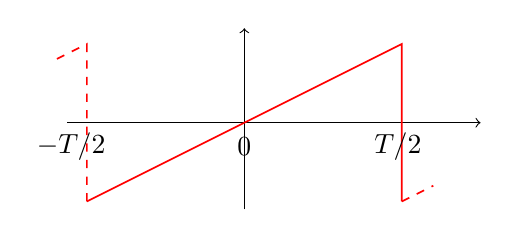
\begin{tikzpicture}[baseline=0mm] 
        \draw[->] (-2.25, 0) -- (3, 0);
        \draw[->] ( 0,-1.1) -- (0, 1.2);
        \draw[semithick,red] (-2,-1) -- ( 2, 1) -- (2,-1);
        \draw[semithick,red, dashed] (-2,-1) -- (-2, 1) -- (-2.4, 0.8);
        \draw[semithick,red, dashed] ( 2,-1) -- ( 2.4,-0.8);
        \draw (-2.2,-0.3) node {$-T/2$};
        \draw ( 0,-0.3) node {$0$};
        \draw ( 1.95,-0.3) node {$T/2$};
    \end{tikzpicture}

\begin{solution}
\begin{minipage}[c]{.49\linewidth}
 \begin{align*}
     a(t) &= ct \\
     c &= \frac{2a_{max}}{T} \\
     \tilde{w}_k &= \frac{2\pi k}{T}
 \end{align*}
 \end{minipage}
 
 \textbf{\raggedright Darstellung der Anregung als Fourierreihe ($N=2$)}

\vspace{1em}

     \begin{align*}
        \intertext{\flushleft Benötigte Integrale:}
        \int x \sin(ax) \dd{x} &= \frac{\sin(ax) - x \cos(ax)}{a} \\
        \int x \cos(ax) \dd{x} &= \frac{\cos(ax) + x \sin(ax)}{a}
     \end{align*}
\dotfill
 \begin{align*}
     A_0 &=  \frac{2}{T} \int\limits_{-\frac{T}{2}}^{\frac{T}{2}} a(t)\dd{t} = \frac{2}{T} \int\limits_{-\frac{T}{2}}^{\frac{T}{2}} ct \dd{t} = \frac{2}{T} \,\Big|\, \frac{c}{2}t^2\,\Big|_{t = -\frac{T}{2}}^{\frac{T}{2}} = \uuline{0}\\
     A_k &= \frac{2}{T} \int\limits_{-\frac{T}{2}}^{\frac{T}{2}} a(t) \cos(\overbrace{\frac{2\pi k}{T}}^{\tilde{w}_k}t)\dd{t} = \frac{2}{T} \int\limits_{-\frac{T}{2}}^{\frac{T}{2}} ct \cos(\tilde{w}_k t) \dd{t} \\
     &= \frac{2}{T} \,\Big|\,\frac{c}{\tilde{w}_k} (\cos(\tilde{w}_k t) + t \sin(\tilde{w}_k t))\,\Big|_{t = -\frac{T}{2}}^{\frac{T}{2}} = \uuline{0}
 \end{align*} 
 %\newpage
 
\begin{minipage}[t]{.49\linewidth}

$\cos(\tilde{w}_k t)$\\

    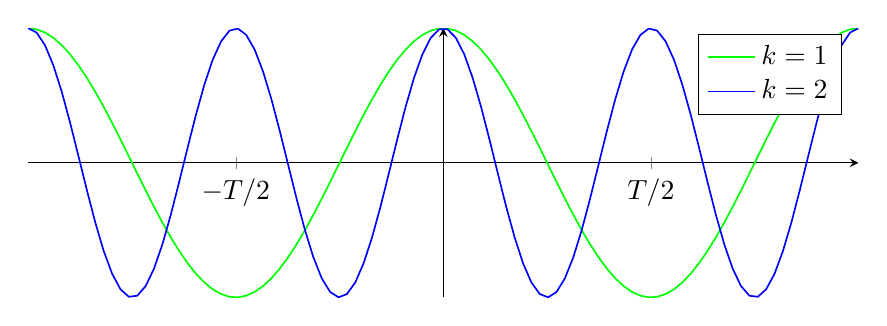
\begin{tikzpicture}
        \begin{axis}[
            width = \linewidth,
            height = 5cm,
            axis x line=center, 
            axis y line=middle, 
            samples=100,
            ymin=-1, ymax=1,
            xmin=-pi, xmax=pi,
            ytick=\empty,
            xtick={-pi/2,pi/2},
            xticklabels={$-T/2$,$T/2$}
            ]
            \addplot [semithick, green, domain=-pi:pi] {cos(2*deg(x))};
            \addlegendentry{$k=1$};
            \addplot [semithick, blue, domain=-pi:pi] {cos(4*deg(x))};
            \addlegendentry{$k=2$};
        \end{axis}
    \end{tikzpicture}
    \end{minipage}
    \begin{minipage}[t]{.49\linewidth}
    
    $\sin(\tilde{w}_k t)$\\
    
    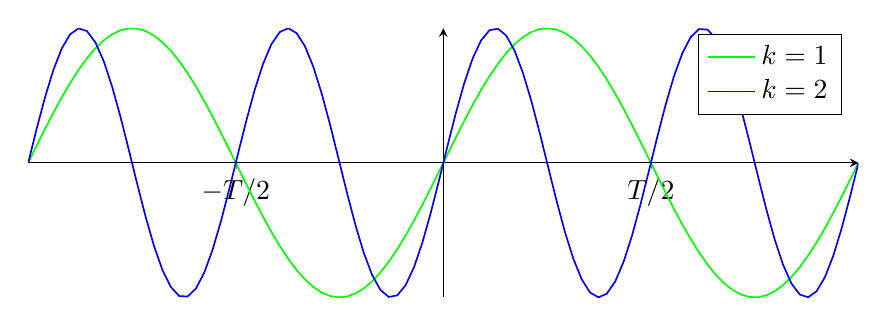
\begin{tikzpicture}
        \begin{axis}[
            width = \linewidth,
            height = 5cm,
            axis x line=center, 
            axis y line=middle, 
            samples=100,
            ymin=-1, ymax=1,
            xmin=-pi, xmax=pi,
            ytick = \empty,
            xtick={-pi/2,pi/2},
            xticklabels={$-T/2$,$T/2$}
            %legend style={draw=none}
            ]
            \addplot [semithick, green, domain=-pi:pi] {sin(2*deg(x))};
            \addlegendentry{$k=1$};
            \addplot [semithick, blue, domain=-pi:pi] {sin(4*deg(x))};
            \addlegendentry{$k=2$};
        \end{axis}
    \end{tikzpicture}
    \end{minipage}
 \vspace{1em}
 
    \begin{align*}
     B_k &= \frac{2}{T} \int\limits_{-\frac{2}{T}}^{\frac{2}{T}} ct \sin(\tilde{w}_k t) \dd{t} = \frac{2}{T}\,\Big|\, \frac{c}{\tilde{w}_k}(\sin(\tilde{w}_k t)-t\cos(\tilde{w}_k t))\,\Big|_{t={-\frac{2}{T}}}^{t=\frac{2}{t}} \\
     &= \frac{-2c}{\tilde{w}_k} \cos(\tilde{w}_k\frac{T}{2}) = 
     \left\{
     \begin{array}{lll}
     \cfrac{2c}{\tilde{w}_k} & &k = 1,3,5,\dots\\[1em]
     -\cfrac{2c}{\tilde{w}_k} & &k = 2,4,6,\dots 
     \end{array}\right.
\end{align*}
\begin{align*}
     \begin{array}{lcl}
        a = \overbrace{B_1\sin(\tilde{w}_1 t)}^{a_1(t)} + \overbrace{B_1\sin(\tilde{w}_2 t)}^{a_2(t)} & \rightsquigarrow & u_p(t) = u_{p1}(t) + u_{p2}(t) \\[1em]
        B_1 = \cfrac{4a_{max}\cancel{T}}{2\pi\cancel{T}} \qquad \tilde{w}_1 = \cfrac{2\pi}{T} && u_{p1}^{(t)} = u_{C1} \cos(\tilde{w}_k t) + u_{S1} \sin(\tilde{w}_1 t) \\[1em]
        B_2 = \cfrac{4a_{max}}{4\pi} \qquad \tilde{w}_2 = \cfrac{4\pi}{T}&& \underbrace{u_{p2}^{(t)} = u_{C2} \cos(\tilde{w}_k t) + u_{S2} \sin(\tilde{w}_2 t)} \\
        &&\text{Partikuläre Lösung - siehe Übung}\\
        &&\text{harmonisch erregte Einmassenschwinger}
        \end{array}
\end{align*}\\[2em]
 
 \textbf{Anpassung der Gesamtlösung an die Anfangsbedingungen}

    \begin{align*}
    u(t_0) &= u_0 \quad,\quad \dot{u}(t_0) = \dot{u}_0\\
    u_0 &= C_1\cos(w_1 t_0)e^{-\delta t_0} + C_2 \sin(w_1 t_0)e^{-\delta t_0} + u_p(t_0)\\
    \intertext{\flushleft Lineares Gleichungssystem der Struktur:}
    &\qquad \begin{bmatrix}
     A_{11} & A_{12}\\
     A_{21} & A_{22}
    \end{bmatrix} 
    \begin{bmatrix}
     C_1 \\ 
     C_2
    \end{bmatrix}
    =
    \begin{bmatrix}
    b_1 \\
    b_2
    \end{bmatrix} \\[1em]
    &\begin{bmatrix}
    C_1 \\
    C_2
    \end{bmatrix}
    = \cfrac{1}{A_{11}A_{22}-A_{12}A_{21}}
    \begin{bmatrix}
     A_{22} & -A_{12}\\
     -A_{21} & A_{11}
    \end{bmatrix}
    \begin{bmatrix}
     b_1 \\
     b_2
    \end{bmatrix}\\
 \end{align*}
\end{solution}

%%% Vorlesung 4 - Dämpfungsmodellierung %%%%
\raggedright

\subsection{Dämpfungsmodellierung}

 \question{Dämpfungskapazität des äquivalent-linearen Modells}
 \vspace{1em}
 
    \begin{minipage}[t]{.49\linewidth}
    geg.:
    \begin{tasks}(1)
      \task[] $F_D = 2\, \zeta\, \nu\, k\, \hat u\, \sin(a\, t)$
      \task[] $\dot{u} = \omega\,\hat\, u\, \sin(a\,t)$
    \end{tasks}
    \end{minipage}
    \begin{minipage}[t]{.49\linewidth}
    ges.:
        \begin{tasks}
            \task dissipierte Energe $\Delta W$ pro Zyklus
            \task maximal in Feder gespeicherte Engerie $W$
            \task Dämpfungskapazität $\Psi$
        \end{tasks}
    \end{minipage}
\vspace{1cm}

 \question{Schubmodul und Dämpfung bei mittleren Dehnungen}
  \vspace{1em}
 
     \begin{minipage}[t]{.49\linewidth}
    geg.:
    \begin{tasks}(1)
      \task[] $\hat\gamma = 0,5\%$
      \task[] $I_p = 10 \%$
    \end{tasks}
    \end{minipage}
    \begin{minipage}[t]{.49\linewidth}
    ges.:
        \begin{tasks}
            \task $-\cfrac{G}{G_{max}}$
            \task $D$
        \end{tasks}
    \end{minipage}
    
    \begin{center}\fbox{\underline{Hinweis:} Kap. 4.2.4 aus Grundbau-Taschenbuch, siehe Scan}\end{center}

\vspace{1cm}

 \question{Schubmodul bei sehr kleinen Dehnungen}
  \vspace{1em}
 
     \begin{minipage}[t]{.49\linewidth}
    geg.:
    \begin{tasks}(2)
      \task[] $e = 2,0$
    \task[] $I_p = 0,6$
    \task[] $P_a = 100 kPa$
    \task[] $\bar \sigma' = 1 MPa$
    \task[] $OCR = 5$
    \end{tasks}
    \end{minipage}
    \begin{minipage}[t]{.49\linewidth}
    ges.:
        \begin{tasks}
            \task $- G_{max|NC}$
            \task $- G_{max|OC}$
        \end{tasks}
    \end{minipage}
 \begin{center}\fbox{\underline{Hinweis:} Kap. 4.2.4 aus Grundbau-Taschenbuch, siehe Scan}\end{center}

 \question{Masing-Hypothese, geometrische Konstruktion}
 \vspace{1em}
 \begin{tasks}
 \task Zeichnen sie die Skelettkurve (punktweise Berechnung).
\task Konstruieren sie für $\cfrac{\hat \gamma}{\gamma_r}=2$ (Faktor 2) die Hysterese-Äste.
 \end{tasks}
 \begin{align*}
 \cfrac{\tau}{\tau_m} = \cfrac{\cfrac{\gamma}{\gamma_r}}{1+|\cfrac{\gamma}{\gamma_r}|}    
 \end{align*}
    \begin{figure}[!h]
        \centering
    \begin{gnuplot}[terminal=epslatex, terminaloptions={size 15cm,10cm}]
        set xr [-10:10]
        set yr [-1:1]
        set xl '$\cfrac{\cfrac{\gamma}{\gamma_r}}{1+|\cfrac{\gamma}{\gamma_r}|}$' offset 0,-2
        set yl '$\frac{\tau}{\tau_r}$' 
        unset key
        set grid
        set zeroaxis
        set title 'Skelettkurve'
        plot x/((1+abs(x)))
    \end{gnuplot}
        \label{fig:Skelettkurve}
        \vfill
    \end{figure}
    
    \newpage
   
    \begin{figure}[!ht]
    \centering
        \begin{minipage}[t]{\textwidth}
        \centering
            \begin{gnuplot}[terminal=epslatex,terminaloptions={size 15cm,18cm}]
                set key off
                set zeroaxis
                set grid
                set yrange [-1:1]
                set multiplot layout 2,1 rowsfirst
                
                set title 'zentrische Streckung der Skelettkurve'
                plot 1/0 
                
                set title 'Spiegelung am Koordinatenursprung'
                plot 1/0 
                
                unset multiplot
            \end{gnuplot}
        \end{minipage}
    \end{figure}
    
\newpage

\section{Wellenausbreitung in 1D, Dehnstab, Rand-/Übergangsbedingungen}

\question{Ein Pfeil wird auf eine Zielscheibe geschossen und bleibt stecken. Warum fliegt das Endstück Rückwärts weg?}

\begin{tasks}(1)
    \task[$\bullet$] Skizzieren Sie den Kraft- und Geschwindigkeitsverlauf im Pfeil (Dehnstab)
    \task[$\bullet$] Vergleichen sie Ihr Ergebnis mit einem Einmassenschwinger, der gegen die Wand fliegt.
\end{tasks}

\begin{solution}
\flushleft HIER BITTE NOCH LÖSUNG NACHTRAGEN
\end{solution}

\question{Ein halbunendlicher Stab wird am Rand harmonisch angeregt. 

\vspace{1cm}

\begin{figure}[h]
    \centering
    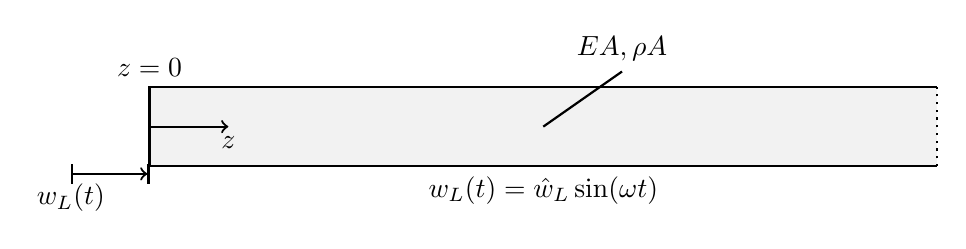
\begin{tikzpicture}
        \draw[thick, fill=gray!10] (10,0) -- node [midway, below] {$w_L (t) = \hat{w}_L \sin(\omega t)$} (0,0) -- (0,1) node[above] {$z=0$} -- (10,1) ;
        \draw[thick, dotted] (10,0) -- (10,1);
        %\draw[thick, ->] (10,0.5) -- (11,0.5);
        \draw[thick, ->] (0,0.5) -- (1,0.5) node[left, below] {$z$} ;
        \draw[thick, |->|] (-1,-0.1) node[below] {$w_L (t)$} -- (0,-0.10);
        \draw[thick] (5,0.5) -- (6,1.2) node[above] {$EA,\rho A$};
    \end{tikzpicture}
\end{figure}

Am Anfang $(t=0)$ ist er undeformiert und in Ruhe. Lösen Sie diese Aufgabe, indem Sie auf dem gedanklich über den Rand verlängerten Stab eine nach rechts laufende Welle annehmen, welche genau die vorgegebene Randbewegung erzeugt. Interpretieren Sie die Parameter dieses Verlaufs physikalisch, Stichwort "Wellenlänge".
}

\begin{solution}
\flushleft HIER BITTE NOCH LÖSUNG NACHTRAGEN
\end{solution}

\question{Berechnen Sie das Reflektionsverhalten diskreter Elemente am Rand: Feder, Dämpfer und Masse.
\begin{figure}[h]
    \centering
    \begin{tikzpicture}
        
    \end{tikzpicture}
\end{figure}

\todo{Bilder einfügen}

Nehmen Sie dazu eine einfallende nach links laufende Welle $w_{ein}(z,t) = C_1 \cos(kz+\omega t)$ an und berechnen Sie die reflektierende Welle $w_{ref}(z,t)=R_1\cos(kz-\omega t) + R_2 \sin(kz-\omega t)$.
}\\[2em]

\fbox{Hinweis ($z=0$):}
\begin{tasks}(3)
    \task[] $kw = EAw''$ 
    \task[] $c\dot w = EAw'$
    \task[] $m\ddot w = EAw'$
    \task[] Feder-RB
    \task[] Dämpfer-RB
    \task[] Masse-RB
\end{tasks}

\end{questions}


\end{document}
